\section{Quantum Error Detection and Correction - 量子错误探测与改正}
\subsection{Classical Error Correction}
The fundamental idea of error detection and correction is to \impt{add redundancy to data to project against errors}. \\
The simplest classical code is ``repetition code'', where we code $0$ as $000$ and $1$ as $111$. We can detect and correct any single bit flip. The rate of this method is $\frac{1}{3}$. \\
Another classical method is the Hamming code, where we code $4$ bits into $7$ bits, with the rate of $\frac{4}{7}$. This is achieved by
$$p_1 = d_1 \oplus d_2 \oplus d_3$$
for one of the error detection code. \\

\subsection{Quantum Error Detection and Correction}
A na\"ive generalization of the repetition code does not work in quantum, the operation:
$$\ketpsi \mapsto \ketpsi\ketpsi\ketpsi$$
is not possible to due \impt{no-cloning principle}.
\begin{definition}
    A $d$-dimensional \uimpt{observable} $\mathcal{O}$ is a $d \times d$ \impt{Hermitian} matrix where $\conjt{\mathcal{O}} = \mathcal{O}$.
\end{definition}
An $n$-qubit observable is a $2^n$-dimensional observable.
\begin{definition}
    Let $\mathcal{O}$ be an $n$-qubit observable, $\ketpsi$ is an $n$-qubit state, suppose $\mathcal{O}\ketpsi = \lambda\ketpsi$ for some $\lambda \in \R$, then \uimpt{measuring} $\mathcal{O}$ on $\ketpsi$ refers to a process that returns $\lambda$ and the state remains $\ketpsi$.
\end{definition}
\begin{definition}
    An $n$-qubit \uimpt{stabilizer} (Pauli operators) is a $2^n \times 2^n$ matrix of form $P_1 \otimes P_2 \otimes \cdots \otimes P_n$, where $P_i \in \{\id, X, Y, Z\}$
\end{definition}
When we measure a stabilizer on an eigenstate, we will obtain outcomes in $\{+1, -1\}$.
\begin{definition}
    If $A, B$ are complex matrices of same dimensions, we say $A, B$ \uimpt{commute} if $AB = BA$ and \uimpt{anti-commute} if $AB = -BA$.
\end{definition}
This gives that any two stabilizers commute or anti-commute. \\
A set of $k$ stabilizers can be \impt{simultaneously} measured if $\mathcal{S}_i$ commutes with $\mathcal{S}_j$. This is a ``physical interpretation'' of the mathematical fact that a set of commuting diagonalizable matrices can be simultaneously diagonalized.
\begin{lemma}
    Let $\ketpsi$ be an $n$-qubit state and $P$ an $n$-qubit stabilizer, and $\opuni$ an $n$-qubit unitary, if $P\ketpsi = \ketpsi$ ($P$ stabilizes $\ketpsi$), and $P\opuni = \alpha \opuni P$, for $\alpha \in \{+1, -1\}$, then measuring $P$ on $\opuni\ketpsi$ gives outcome $\alpha$.
\end{lemma}

\subsubsection{Bit-flip Error}
Analogous to the repetition code, we encode a state $\ketpsi = \alpha \ket{0} + \beta \ket{1}$ to be $\ket{\psi'} = \alpha\ket{000} + \beta\ket{111}$, where $\ket{000} := \ket{0_L}$ and $\ket{111} = \ket{1_L}$ (``L'': logical encoding). \\
This is achieved through the circuit:
\begin{center}
    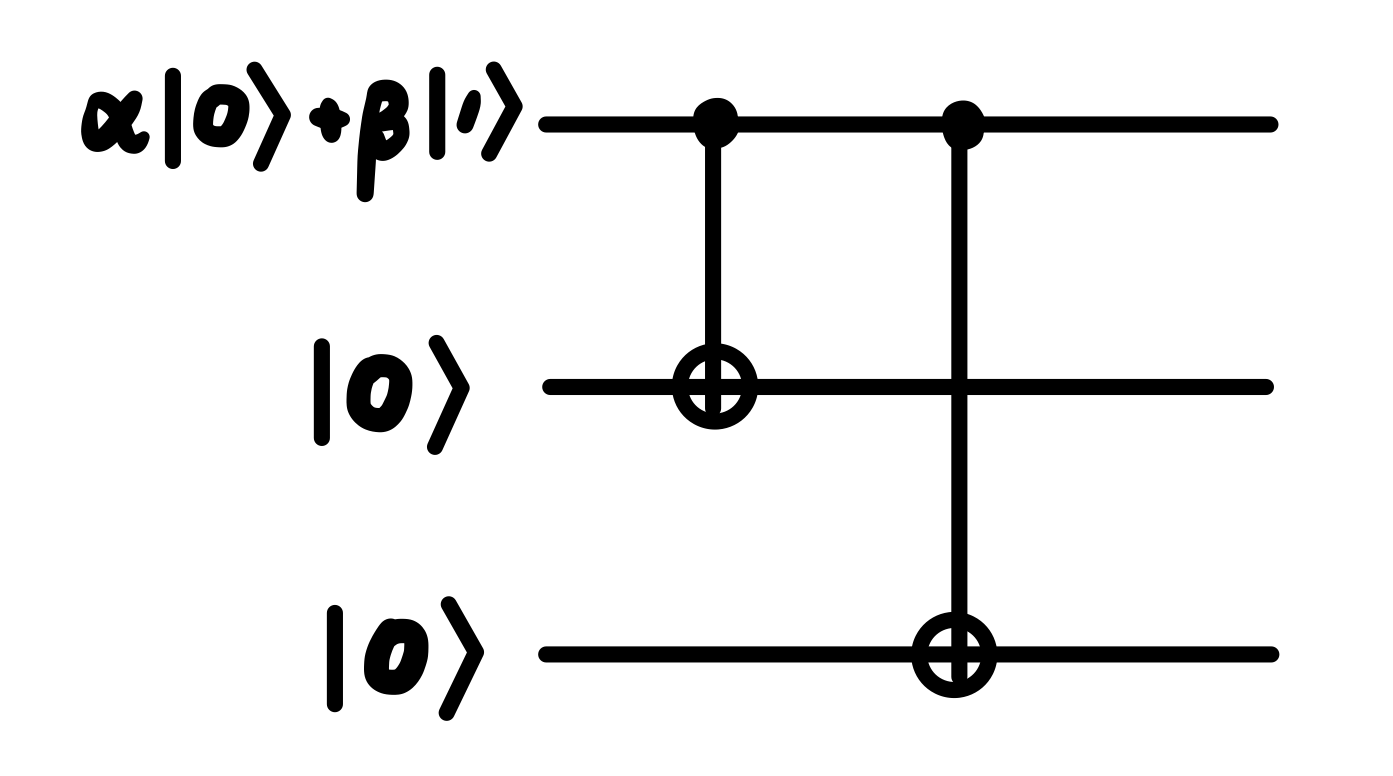
\includegraphics[scale = 0.2]{10/bitflip.png}
\end{center}
This protects against any single-qubit flip. We can detect and correct the errors by measuring:
\begin{align*}
    Z_1Z_2 &= Z \otimes Z \otimes \id \\
    Z_2Z_3 &= \id \otimes Z \otimes Z
\end{align*}
If we measure to $(+, +)$, there is no error. If we measure to $(-, +)$, the first qubit is flipped. If we measure to $(-, -)$, the second qubit is flipped. If we measure to $(+, -)$, the third qubit is flipped. We call this the ``error syndrome table''. \\
However, this cannot detect phase flips.

\subsubsection{Phase-flip Error}
We encode a state $\ketpsi = \alpha \ket{0} + \beta \ket{1}$ to be $\ket{\psi'} = \alpha\ket{+++} + \beta\ket{---}$, where $\ket{+++} := \ket{0_L}$ and $\ket{---} = \ket{1_L}$ through the circuit:
\begin{center}
    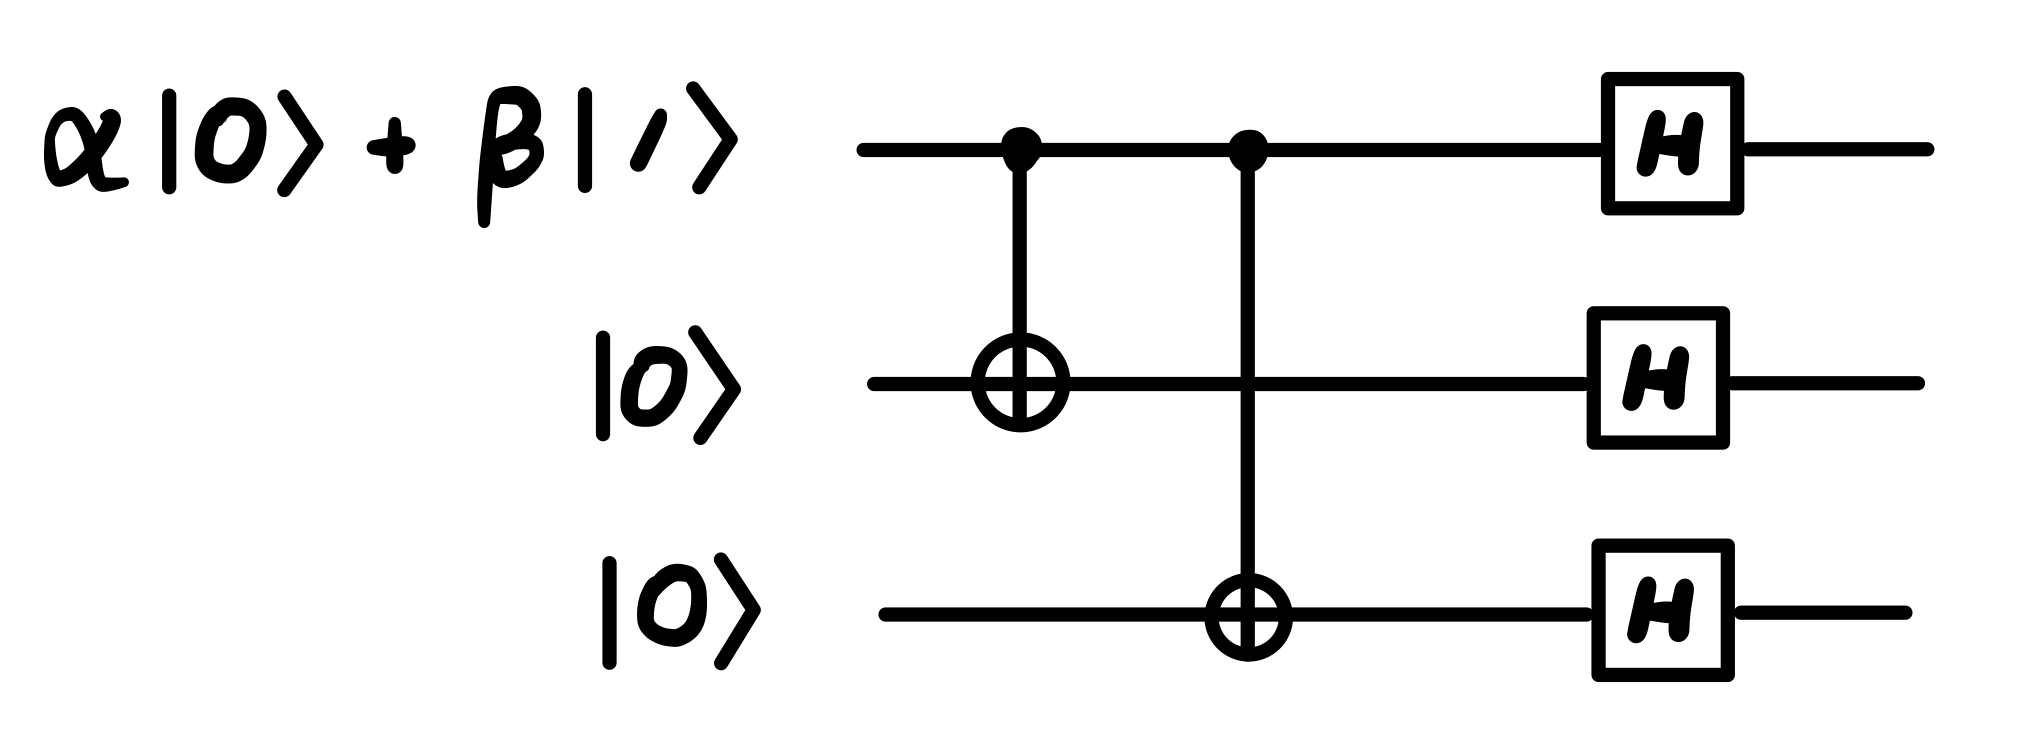
\includegraphics[scale = 0.2]{10/phaseflip.png}
\end{center}
We then measure $(X_1X_2, X_2X_3)$. Analogous to previous section, this can detect any single-qubit phase flip, not any single-qubit bit flip.

\subsubsection{Shor's Code}
One way to detect both bit flips and phase flips on a single-qubit is to use $9$-qubit Shor's code, where it is achieved by the circuit:
\begin{center}
    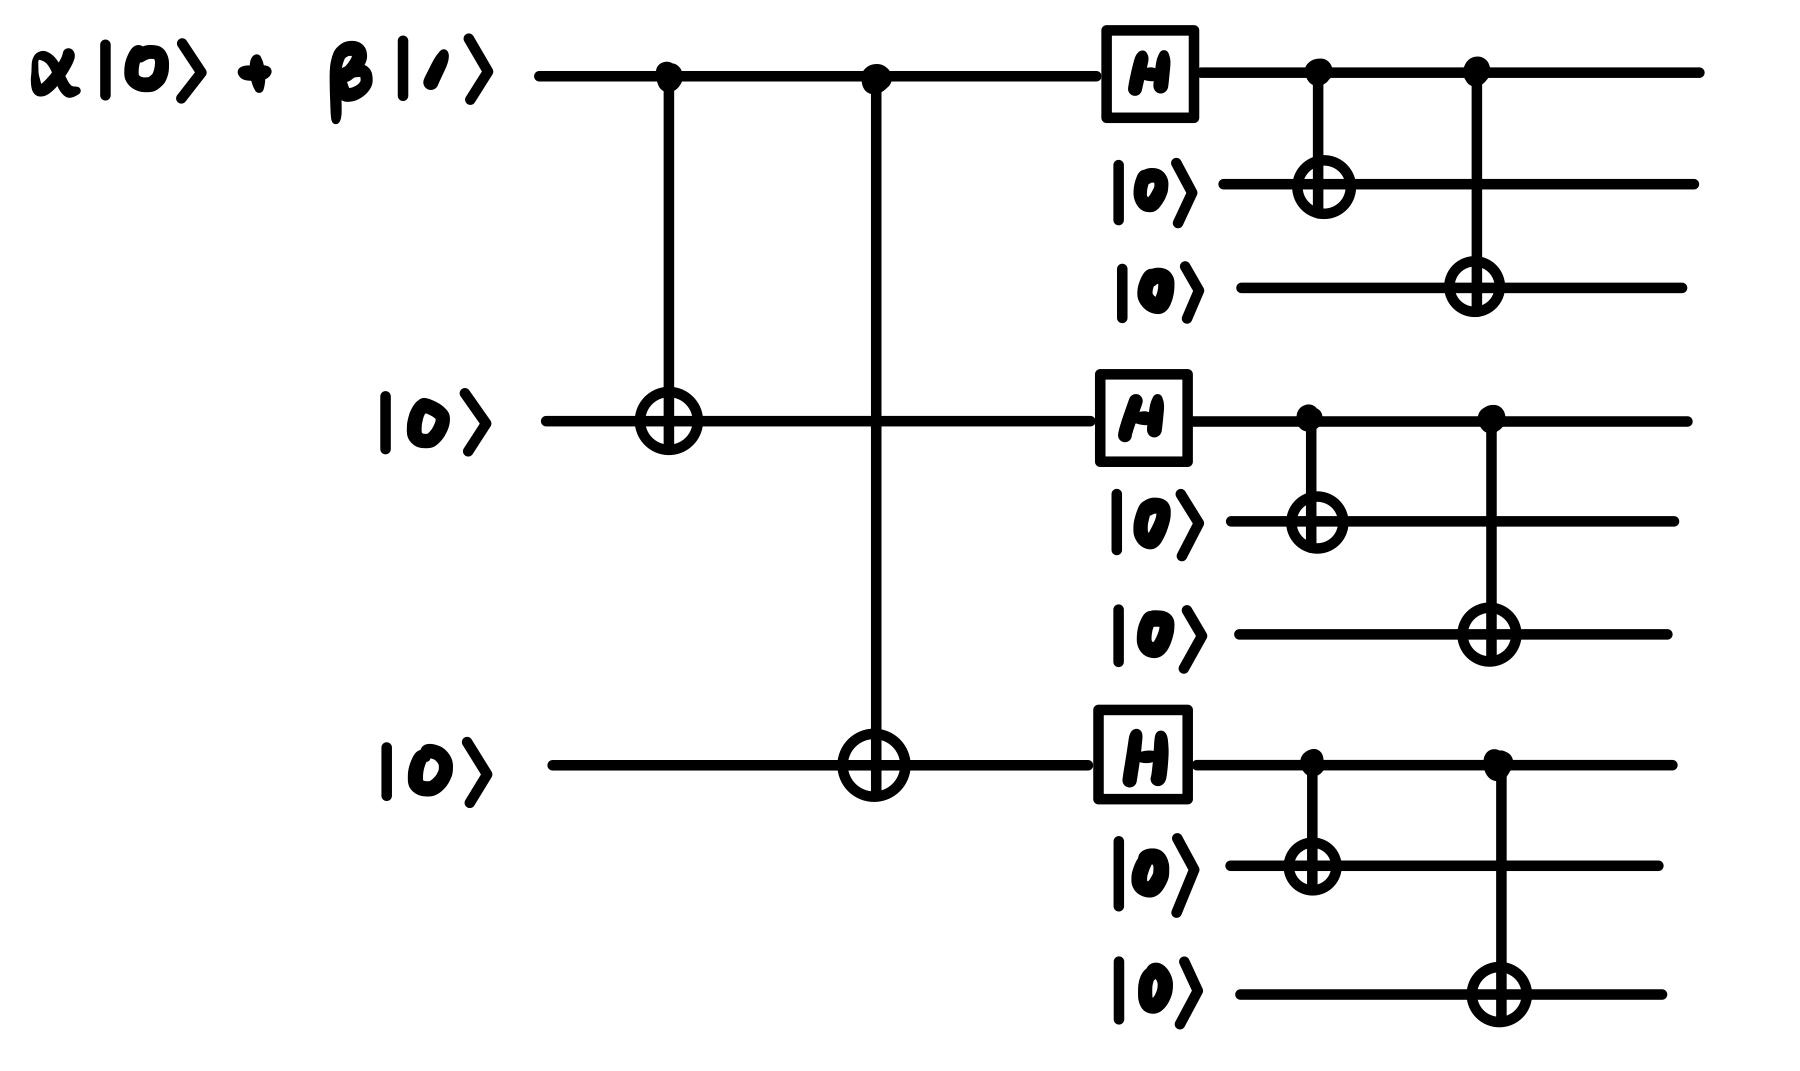
\includegraphics[scale = 0.2]{10/bothflip.png}
\end{center}
And the logical encoding is that
\begin{align*}
    \ket{0_L} &:= \frac{1}{2\sqrt{2}}(\ket{000} + \ket{111})(\ket{000} + \ket{111})(\ket{000} + \ket{111}) \\
    \ket{1_L} &:= \frac{1}{2\sqrt{2}}(\ket{000} - \ket{111})(\ket{000} - \ket{111})(\ket{000} - \ket{111})
\end{align*}
The corresponding stabilizers are:
$$(Z_1Z_2, Z_2Z_3),(Z_4Z_5, Z_5Z_6)(Z_7Z_8, Z_8Z_9)$$
and
$$(X_1X_2X_3X_4X_5X_6, X_4X_5X_6X_7X_8X_9)$$
Even though Shor's code's error syndrome table has non-distinct columns, we can still correct any single qubit error. \\
For example, the columns $Z_1, Z_2, Z_3$ (error gates) will be the same, if we observe the common syndrome of $Z_1, Z_2, Z_3$, we can still correct by multiplying the state by $Z_1$.
\begin{quote}
    1. Error was $Z_1$: $Z_1(Z_1\ketpsi) = \ketpsi$. \\
    2. Error was $Z_2$: $Z_1(Z_2\ketpsi) = (Z_1Z_2)\ketpsi = \ketpsi$ as $Z_1Z_2$ is a stabilizer. \\
    3. Error was $Z_3$: $Z_1(Z_3\ketpsi) = (Z_1Z_2)(Z_2Z_3)\ketpsi = \ketpsi$
\end{quote}
We can identify the block on which the error occurred:
\begin{quote}
    1. if the $Z$ rows have $-$ signs, $1-3$ are the first block, $4-6$ are the second block, and $7-9$ are the third block, with $X, Y$ errors. \\
    2. if the $X$ rows take value $(-, +)$, it's first block; if $(-, -)$, it's second block; if $(+, -)$, it's third block.
\end{quote}
If a QEC can correct any single-qubit $X,Y,Z$ errors, then it can correct ``arbitrary'' single-qubit errors.

\subsection{How to Measure Stabilizers}
We can measure say $\id \otimes X \otimes Y \otimes Z$ on a $4$-qubit state $\ketpsi$ in the following way:
\begin{center}
    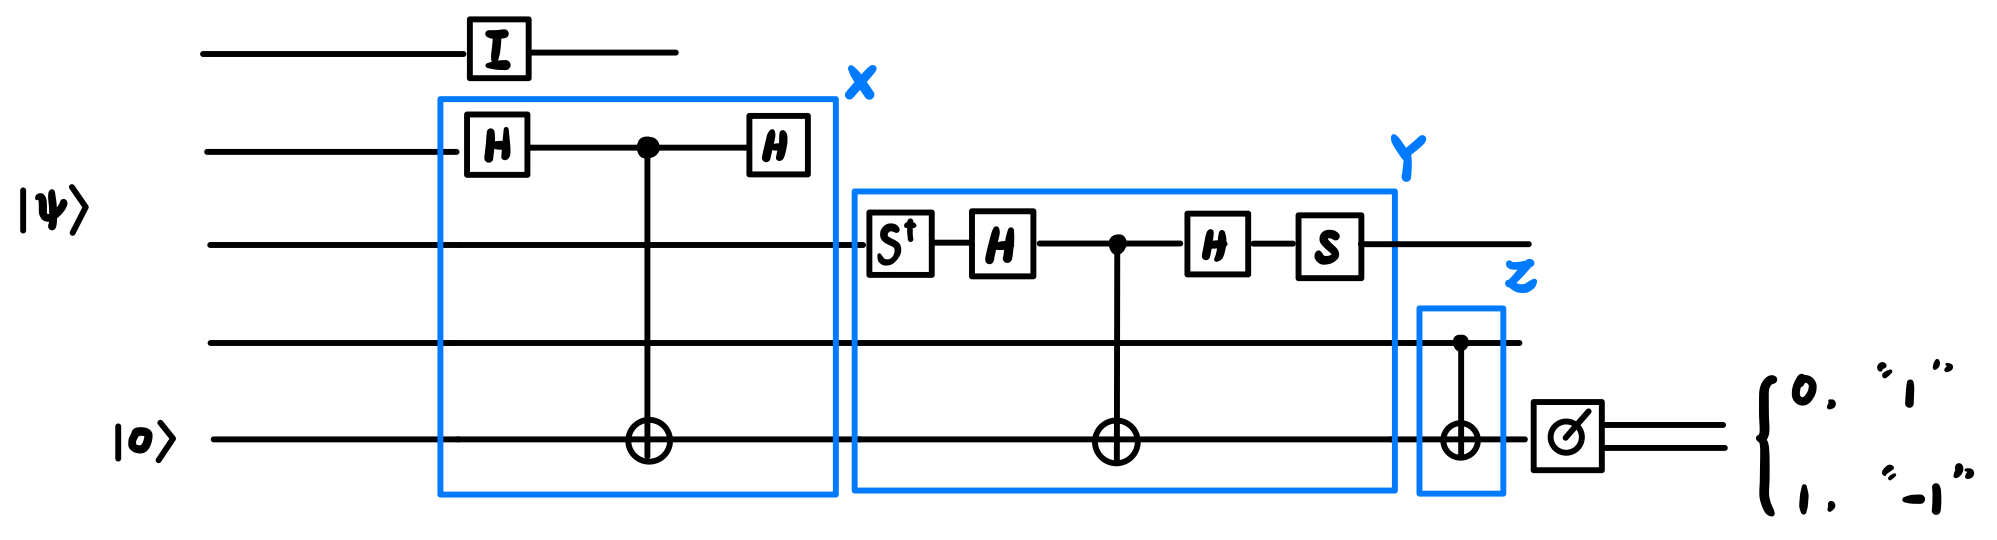
\includegraphics[scale = 0.2]{10/stabilizer.png}
\end{center}